% Created 2018-05-09 Wed 14:49
% Intended LaTeX compiler: xelatex
\documentclass[a4paper,11pt]{article}
\usepackage{graphicx}
\usepackage{grffile}
\usepackage{longtable}
\usepackage{wrapfig}
\usepackage{rotating}
\usepackage[normalem]{ulem}
\usepackage{amsmath}
\usepackage{textcomp}
\usepackage{amssymb}
\usepackage{capt-of}
\usepackage{hyperref}
\usepackage{ctex}
\setCJKmainfont{SimSun}
\author{骆炜}
\date{\today}
\title{猫狗大战(最终篇)}
\hypersetup{
 pdfauthor={骆炜},
 pdftitle={猫狗大战(最终篇)},
 pdfkeywords={},
 pdfsubject={},
 pdfcreator={Emacs 25.3.1 (Org mode 9.1.12)}, 
 pdflang={English}}
\begin{document}

\maketitle
\tableofcontents


\section{项目概览}
\label{sec:org5b7cecf}
本项目基于Kaggle公开训练的和测试数据集实现对图像中猫狗进行图像识别。本项目涵盖数据处理,模型选择和搭建以及最终测试等主要步骤。
本项目所涉及的为典型的二分类问题,需要通过训练集的图片对自己所设计的或是改进的神经网络进行训练,而后通过Kaggle官方的评价系统评判所选模型的准确性。相比于对目标图像的判别,这个项目更重视分类的准确性,需要达到Kaggle评分标准(loss不高于0.06127)。

\section{数据研究}
\label{sec:orgf8b2730}
本项目有Kaggle提供了25000张训练照片和12500测试照片。对于数据的研究主要针对训练照片展开,而测试照片将会原封不动保留到测试步骤。数据的总量较少,因此难以独立完整地训练复杂的卷积神经网络。常见的处理流程包括,数据预筛选,数据增强等。这些处理流程的目的是为了尽量减少错误的信息对模型的误导(例如将贴上错误标签的图像用于分类),或是增加可用的训练的数据等。

\subsection{预处理筛除}
\label{sec:org59f6c32}
首先,根据这篇\href{https://github.com/ypwhs/dogs\_vs\_cats}{Github内容}\footnote{\url{https://github.com/ypwhs/dogs\_vs\_cats}}所述的方法创建符号链接,避免复制一遍照片。其次,依据\href{https://zhuanlan.zhihu.com/p/34068451}{这篇博客}\footnote{\url{https://zhuanlan.zhihu.com/p/34068451}}所提示的信息,我也对Kaggle的数据集进行了筛查。所用的方法和博客作者类似,通过已经在ImageNet数据集下进行了训练的模型,对包括猫狗在内的多个类别能进行预先的判断。具体来说,结合时下比较精确的三个的网络模型(如图\ref{fig:keras}所示),ResNet50,Xception和Inception-ResNetV2,共同对原数据集进行预筛查。每个模型最终的结果选择TOP-10作为判断依据,即如果前10个判断中有出现猫/狗相关的判断,即可认为这张图片中存在猫/狗,反之则需要添加到排除列表中。在 \textbf{pre\_check\_img.py} 中有代码的具体实现。最终代码将会将结果以npy文件和txt文件的方式存储结果。npy文件能够方便的在接下来的编程中快速进行结果调用,而txt文件可以很直观的将结果显示出来,部分结果如图\ref{fig:remove}所示。图\ref{fig:missfigure}所示为两种典型的无法通过3种模型判断的照片。图\ref{fig:missfigure}左为标记在猫分类下的训练照片(cat.7920)。虽然人的肉眼可以看到确实有一张黑猫躺在深蓝色的床单上,但是由于对比度比较低,三个模型都没法将其判别,这样的照片很难给之后所需要训练的模型提供正确有用的信息。这张图还有一个特点是右侧的狗非常显眼,如果这张图标记成猫进行训练,很可能对本项目所需判断的猫狗分类产生比较大的干扰,因此需要移除。图\ref{fig:missfigure}右侧的图片被标记为狗(dog.8736),显然这是一个明显错误的标记,因此也需要将图片移出训练集。

\begin{figure}[htb]
\centering
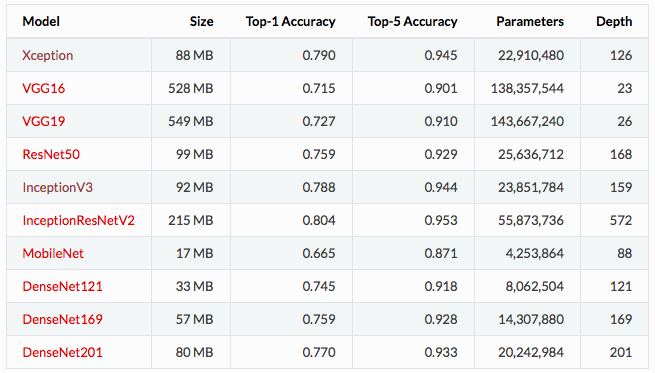
\includegraphics[scale=0.4]{./figure/keras.png}
\caption{当前Keras提供的基于ImageNet训练模型排名}
\label{fig:keras}
\end{figure}

\begin{figure}[htb]
\centering
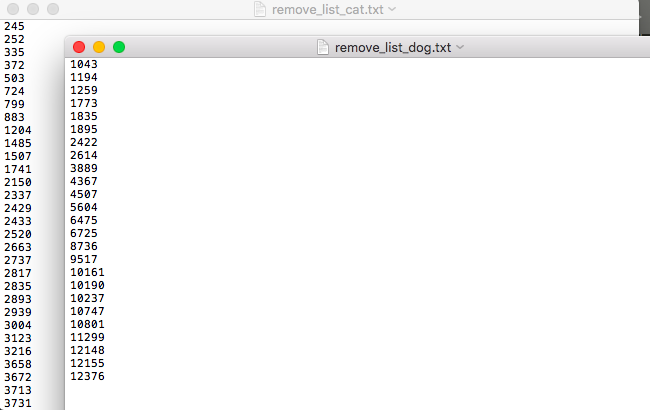
\includegraphics[scale=0.4]{./figure/removelist.png}
\caption{部分需要移除的照片列表}
\label{fig:remove}
\end{figure}

\begin{figure}[htb]
\centering
\subfigure{
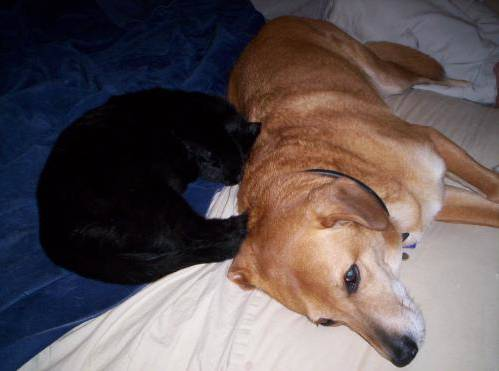
\includegraphics[scale=0.4]{./figure/cat.7920.jpg}
\label{fig:miss1}
}
\subfigure{

\includegraphics[scale=0.4]{./figure/dog.8736.jpg}
\label{fig:miss2}
}
\caption{被移除的部分照片示例}
\label{fig:missfigure}
\end{figure}

\subsection{数据增强}
\label{sec:orgf6aef71}
数据增强是一系列扩充图像数据的方法的统称,通过裁切、添加噪音、改变颜色等手段,对原始照片进行处理,进而生成更多的可用于训练的图像数据,部分地弥补数据量不足造成的过拟合问题,如图\ref{fig:imgaug}。本项目使用Github中开源项目Imgaug\footnote{\url{https://github.com/aleju/imgaug}}进行数据增强的图片生成。Imgaug集成了多种数据增强手段,可以方便的调用。本项目选用了四种手段进行预处理,每张照片选择两个处理手法进行组合,即一张照片最终可以生成六张照片。示例如图\ref{fig:cats}所示。具体的代码实现可查阅两个python文件 \textbf{create\_aug\_fotos.py} 和 \textbf{data\_aug\_tool.py} 。最终通过数据增强算法将通过筛选后的训练文件生成约15万张猫狗照片进行后续的模型训练。

\begin{figure}[htb]
\centering
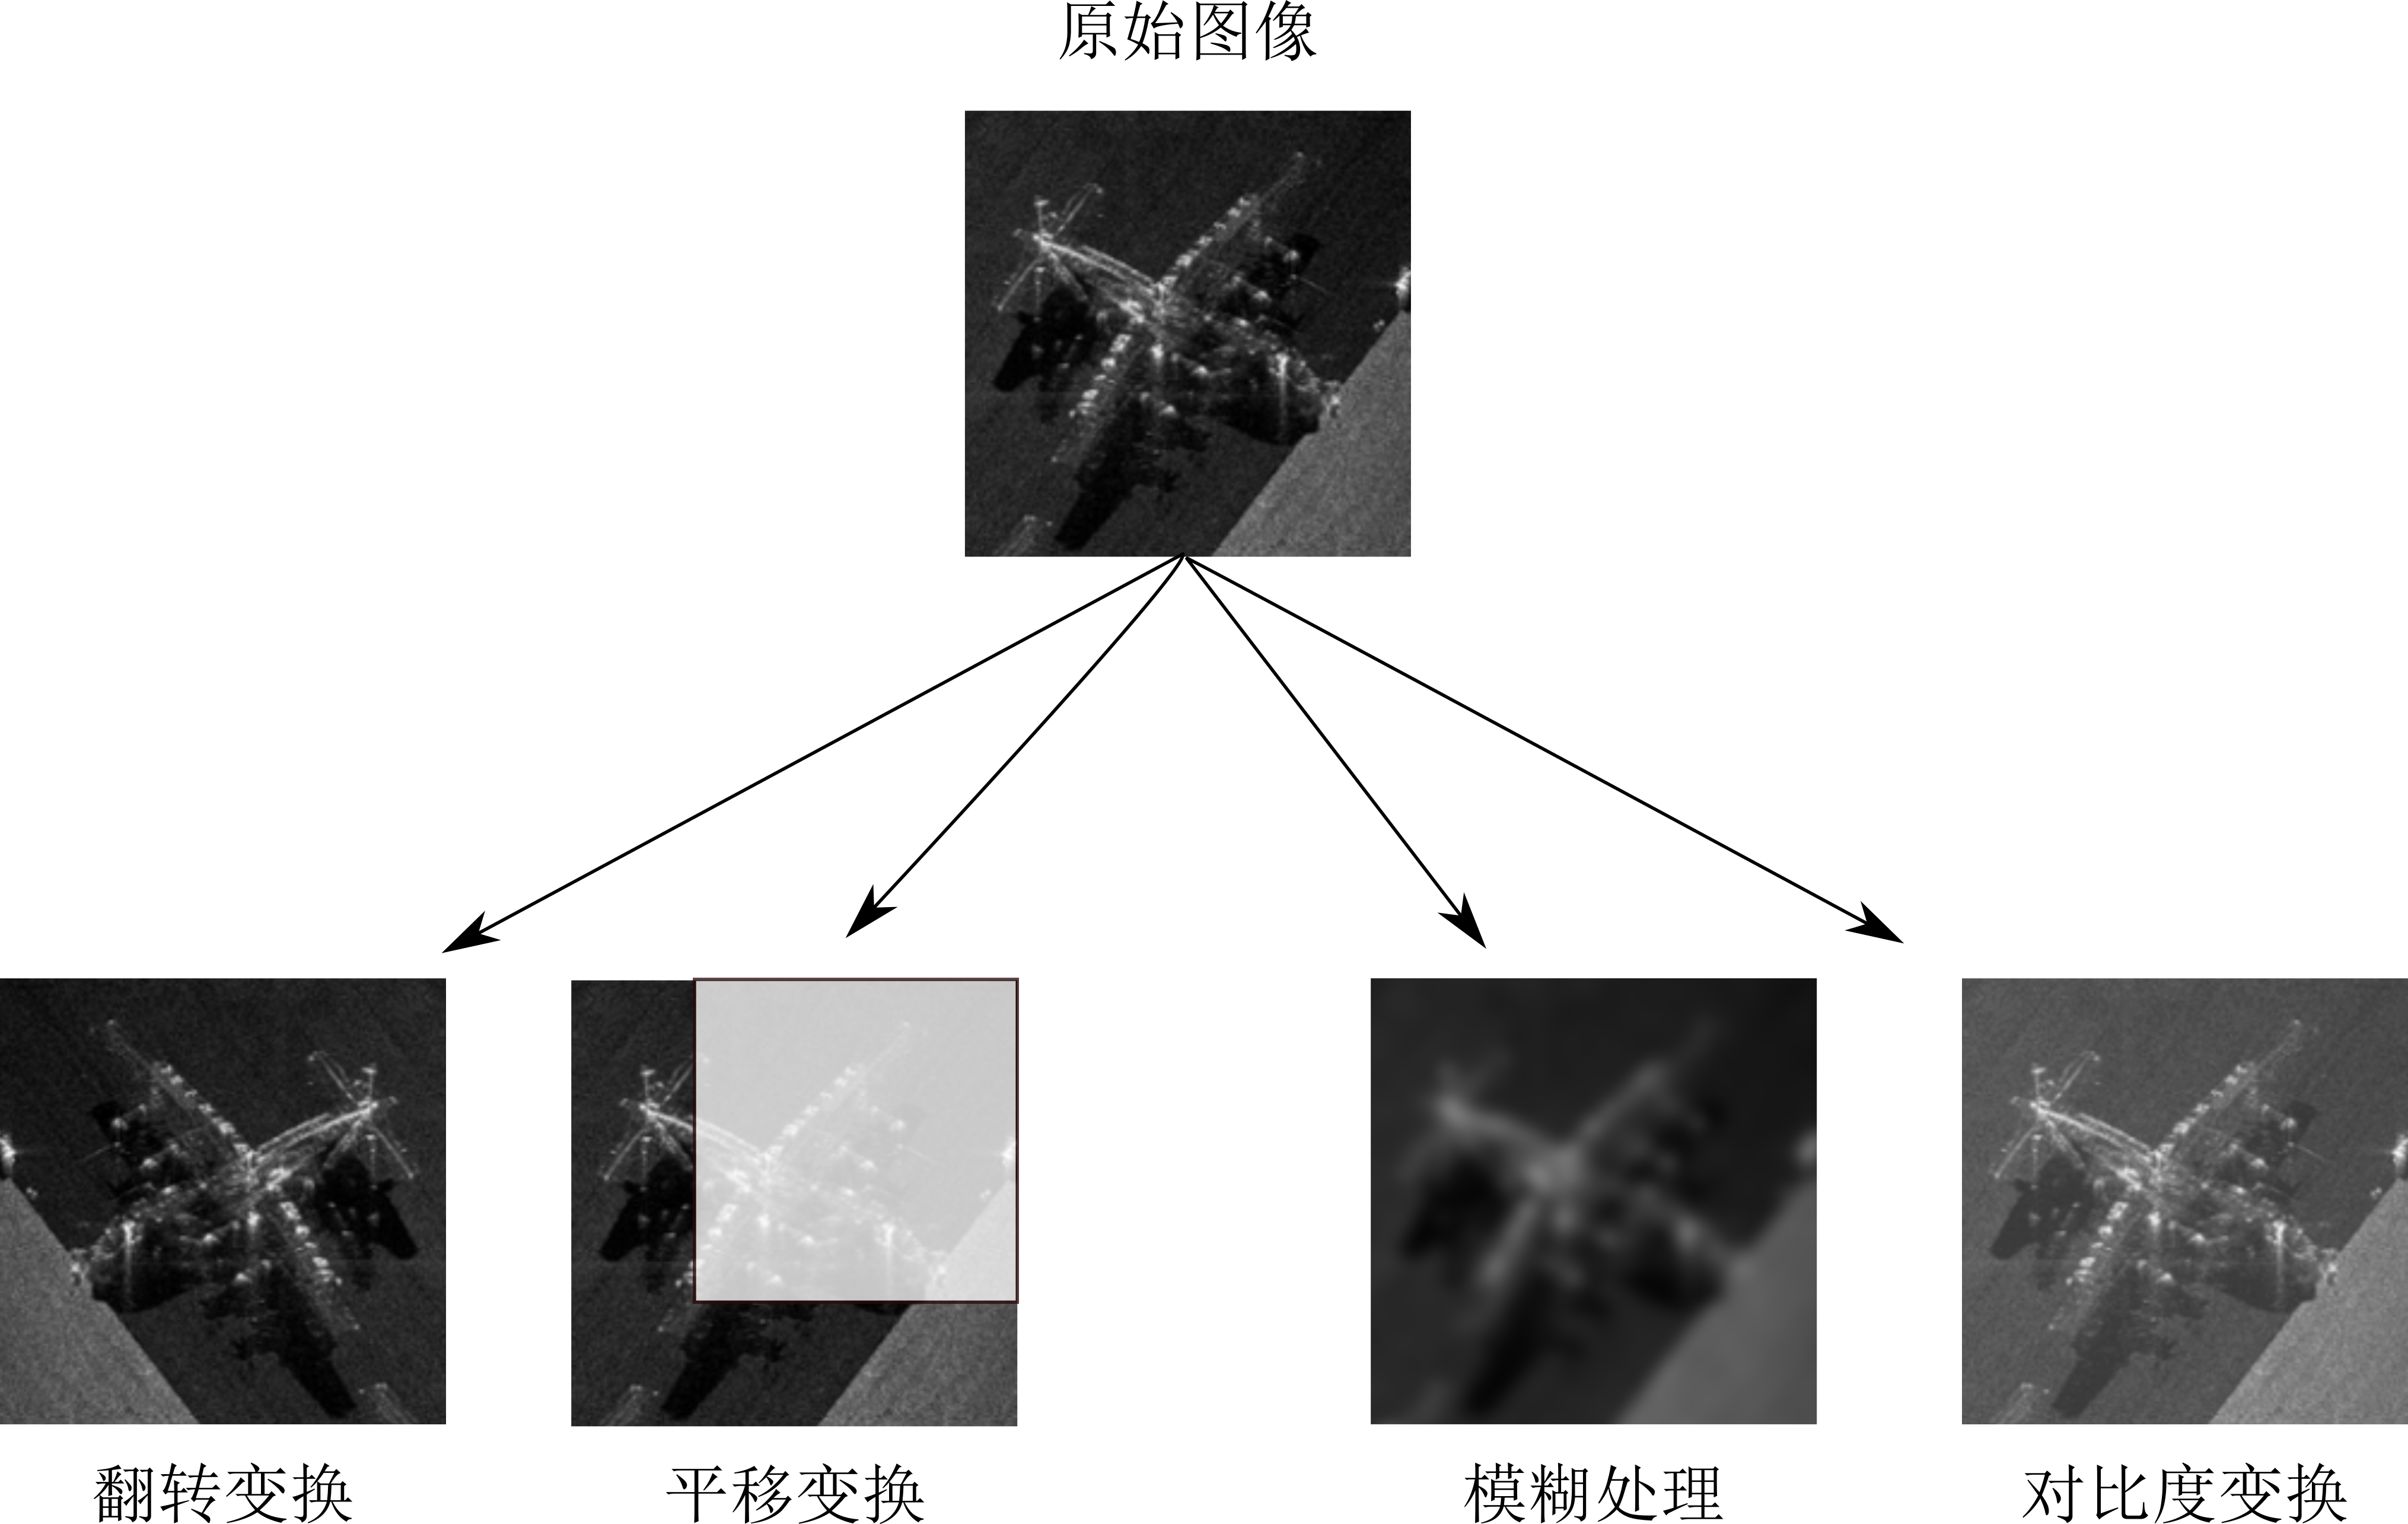
\includegraphics[scale=0.5]{./figure/tuxiang.png}
\caption{数据增强常用的手法}
\label{fig:imgaug}
\end{figure}

\begin{figure}[htb]
\centering
\subfigure{
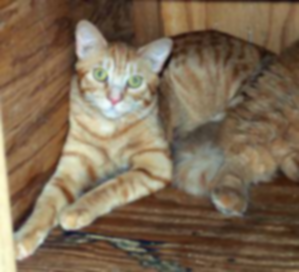
\includegraphics[scale=0.4]{./figure/cat1.jpg}
\label{fig:cat1}
}
\subfigure{
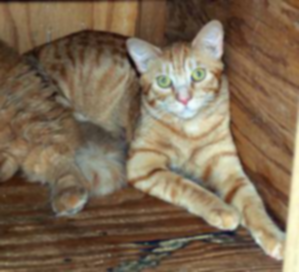
\includegraphics[scale=0.4]{./figure/cat2.jpg}
\label{fig:cat2}
}
\subfigure{
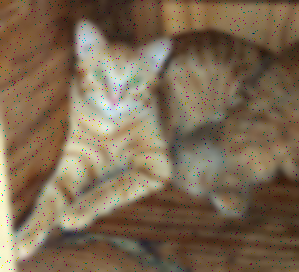
\includegraphics[scale=0.4]{./figure/cat3.jpg}
\label{fig:cat3}
}
\subfigure{
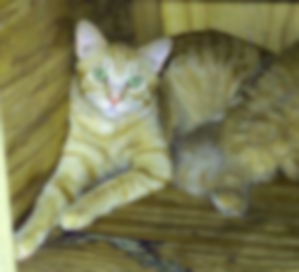
\includegraphics[scale=0.4]{./figure/cat4.jpg}
\label{fig:cat4}
}
\subfigure{
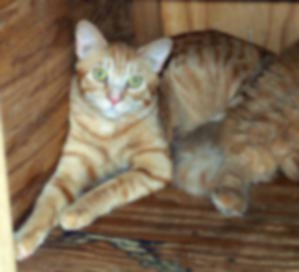
\includegraphics[scale=0.4]{./figure/cat5.jpg}
\label{fig:cat5}
}
\subfigure{
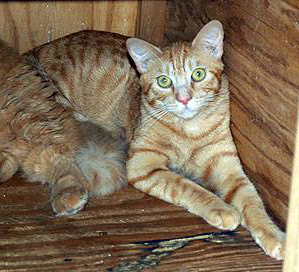
\includegraphics[scale=0.4]{./figure/cat6.jpg}
\label{fig:cat6}
}
\caption{Imgaug处理结果}
\label{fig:cats}
\end{figure}


\section{算法与方法}
\label{sec:org59c1e6b}
由于Keras提供了非常便捷的功能,大部分算法部分的结构不需要自行重新编程。为了提高最终的识别精度,本项目结合了之前预筛选所选用的三种模型进行迁移学习,最后加入自定义的层进行训练。如图\ref{fig:selfmodel}所展现的就是三个模型融合的示意图。通过三个已经预训练好的模型,生成的特征向量的融合,接上相对较为简单的Dropout层,将三个模型的结果融合成最终的判断--猫/狗。

\begin{figure}[htb]
\centering
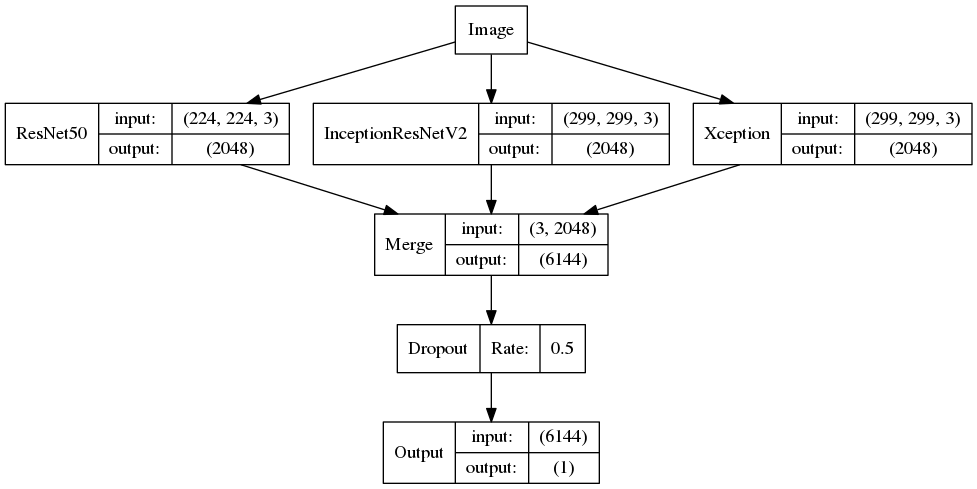
\includegraphics[scale=0.38]{./figure/eg.png}
\caption{自定义的模型结构示意图}
\label{fig:selfmodel}
\end{figure}

\subsection{生成特征向量}
\label{sec:org9685cf3}
使用特征向量和训练数据生成特征向量,有利于快速进行训练。每个选用的模型都将分别根据提供 训练数据生成对应的特征向量。其中使用原始训练数据得到的特征向量.h5文件大约300多MB,而使用数据增强方式生成的照片进行生成的数据文件每个.h5文件大约1.5GB。具体代码详见 \textbf{Feature\_Gen.py} 或是jupyter notebook文件。

\section{测试结果}
\label{sec:org32561f6}
\subsection{测试结果}
\label{sec:org59eb413}
在测试的时候,将预生成好的.h5文件载入,连接上自定义的网络层进行训练,并将结果以Kaggle要求的csv文件方式保存。相较于直接导入数据进行训练,利用特征向量的方法在训练和测试结算所画的时间相对较小,能够很快的完成训练,如图所示。最后将生成的csv文件上传至Kaggle平台,得到如下测试结果,图\ref{fig:kaggle}。满足了项目不大于0.06的需求。

\begin{figure}[htb]
\centering
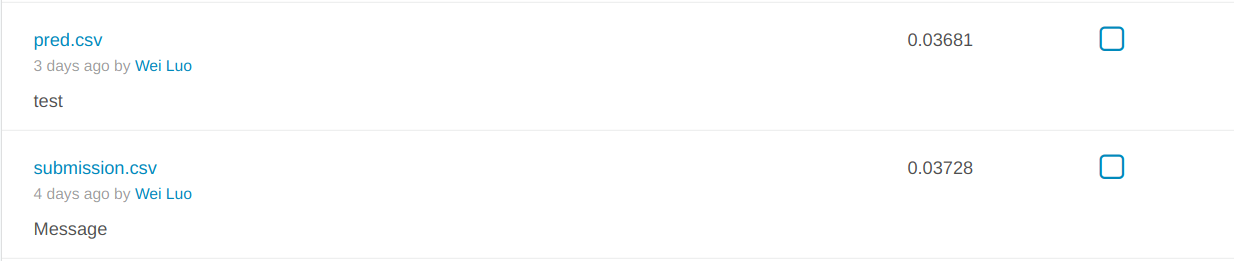
\includegraphics[scale=0.25]{./figure/record.png}
\caption{Kaggle测试结果}
\label{fig:kaggle}
\end{figure}

最终结果为,以数据增强后训练的模型比直接使用原训练数据的模型有较好的测试结果
(0.03681 vs 0.03728)。

通过Tensorboad可以很方便地观察训练过程,其结果如图\ref{fig:tb}所示。由于本身融合
模型已经能够对猫狗进行识别,因此训练的时候起始精度已经非常高,通过较少epoch的训
练,已经能够达到很高精度。整体训练精度变化符合预期,说明模型设置没有明显问题。

\begin{figure}[htb]
\centering
\subfigure{
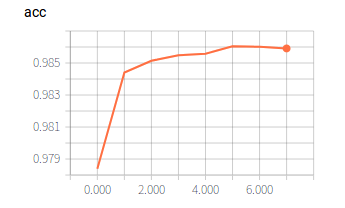
\includegraphics[scale=0.4]{./figure/acc.png}
\label{fig:tb1}
}
\subfigure{
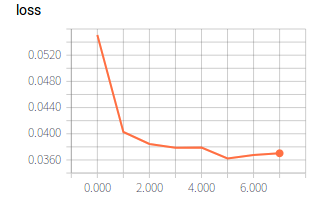
\includegraphics[scale=0.4]{./figure/loss.png}
\label{fig:tb2}
}
\subfigure{
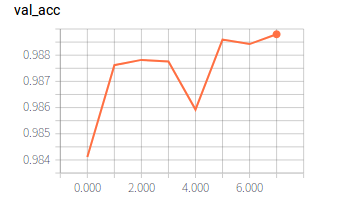
\includegraphics[scale=0.4]{./figure/valacc.png}
\label{fig:tb3}
}
\subfigure{
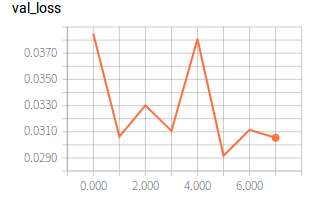
\includegraphics[scale=0.4]{./figure/valloss.png}
\label{fig:tb4}
}
\caption{通过Tensorboard观察的训练过程}
\label{fig:tb}
\end{figure}

\subsection{识别可视化}
\label{sec:orge6b2499}
根据这篇\href{https://github.com/ypwhs/dogs\_vs\_cats}{Github内容}中提示的方法,进行了猫狗识别的可视化。可视化的方法是通过热图的方法对相关区域进行高亮,越是对此类别识别相关的区域,越是会以暖色来显示。具体效果如图\ref{fig:hm}所示。由图所示的结果,首先对于所随机抽样的的图片,模型都能做到准确识别。其次,通过观察我们可以发现,基本上模型用于判断是猫还是狗的区域是猫狗的脸部特征,也就是图片中庸红色或是暖色标记的区域。

\begin{figure}[htb]
\centering
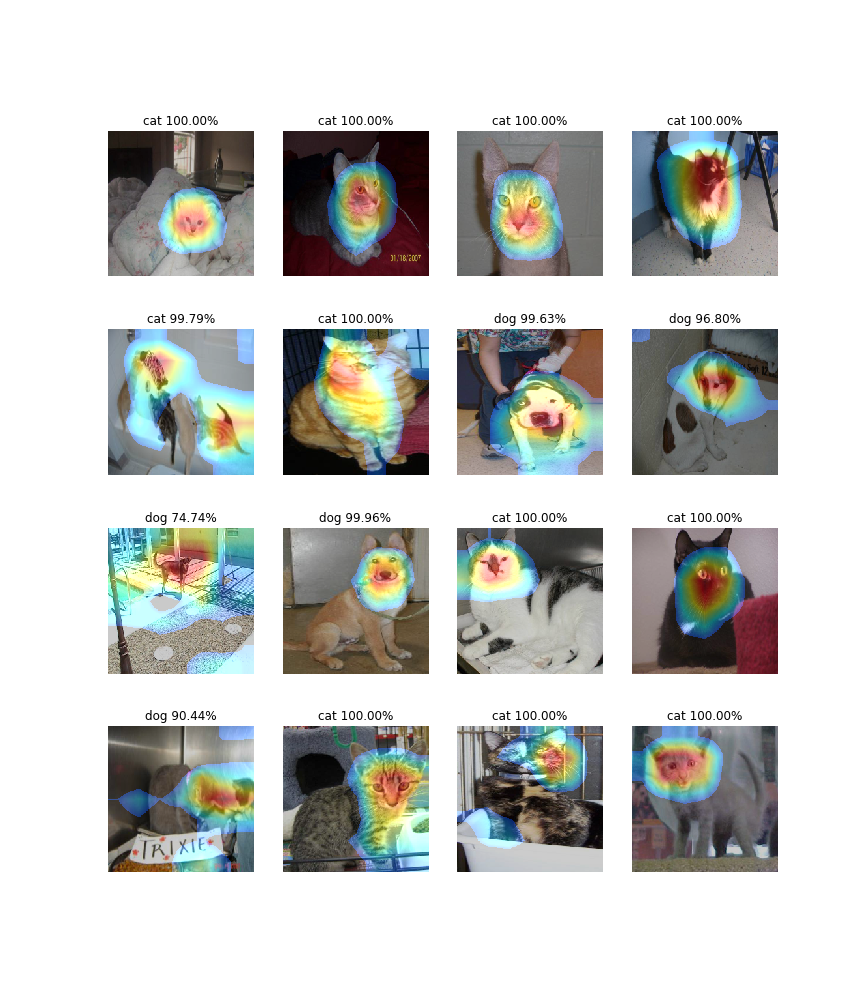
\includegraphics[scale=0.45]{./figure/heatmap.png}
\caption{识别可视化热图}
\label{fig:hm}
\end{figure}

\subsection{需要作出的改进}
\label{sec:org77d173e}
之后结合模型结构优化,可能会取得更好的结果。例如,可以考虑除了去掉各个预训练模型的全连接层外,进一步扩展可训练的模型参数。基于数据增强的方法已经将可用于训练模型的图像数据扩充了很多,因此有希望训练参数更多的模型,这样原本模型的泛用性会进一步降低,可能会取得更好的结果。

\section{项目附件及其说明}
\label{sec:org9417558}

现在对Github提交的文件进行补充说明: 
\begin{enumerate}
\item final\_paper.pdf -- 最终报告文稿
\item create\_symbol\_link/\_2.py -- 生成图像的符号链接
\item pre\_check\_img.py, remove\_list\_cat/dog.txt -- 判断是否非猫非狗
\item create\_aug\_fotos.py data\_aug\_tool.py  -- 数据增强工具
\item Feature\_Gen.py  -- 生成特征向量
\item TrainingandTesting.py -- 训练并获得结果
\item submission\_first/final.csv  -- kaggle提交文件
\item Final\_jupyter\_notebook.ipynb  -- 解释性jupyter notebook
\end{enumerate}
\end{document}